% INTRODUCCIÓN

\cleardoublepage

\chapter{Introducción}
\label{introduccion}

Escribe aquí la introducción de tu Trabajo Fin de Máster, utilizando tantas secciones, subsecciones y subsubsecciones como estimes necesarias.

\section{Mi primera sección}
\label{mi-primera-seccion}

\textbf{Esta palabra} está en negrita. \textit{Esta palabra} está en cursiva. \destacado{Esta palabra} se destaca en púrpura.
\medskip

\section{Mi segunda sección}
\label{mi-segunda-seccion}

En la sección~\ref{mi-primera-seccion} se muestran ejemplos de palabras en negrita, cursiva y destacadas en púrpura.
\medskip

% Define los acrónimos en el fichero secciones/glosario.tex
% Define la bibliografía en el fichero bibliografia.bib
Una \acrfull{gan} es... \citep{goodfellow2014generative}.
\medskip

\citet{goodfellow2014generative} diseñaron las redes generativas antagónicas como...
\medskip

\vspace{5ex}

Listado:
\begin{itemize}
  \item Item 1.
  \item Item 2.
  \item Item 3.
\end{itemize}

Enumeración:
\begin{enumerate}
  \item Item 1.
  \item Item 2.
  \item Item 3.
\end{enumerate}

\subsection{Una subsección}
\label{una-subseccion}

La figura~\ref{fig1} muestra...

\begin{figure}[ht!]
    \centering
    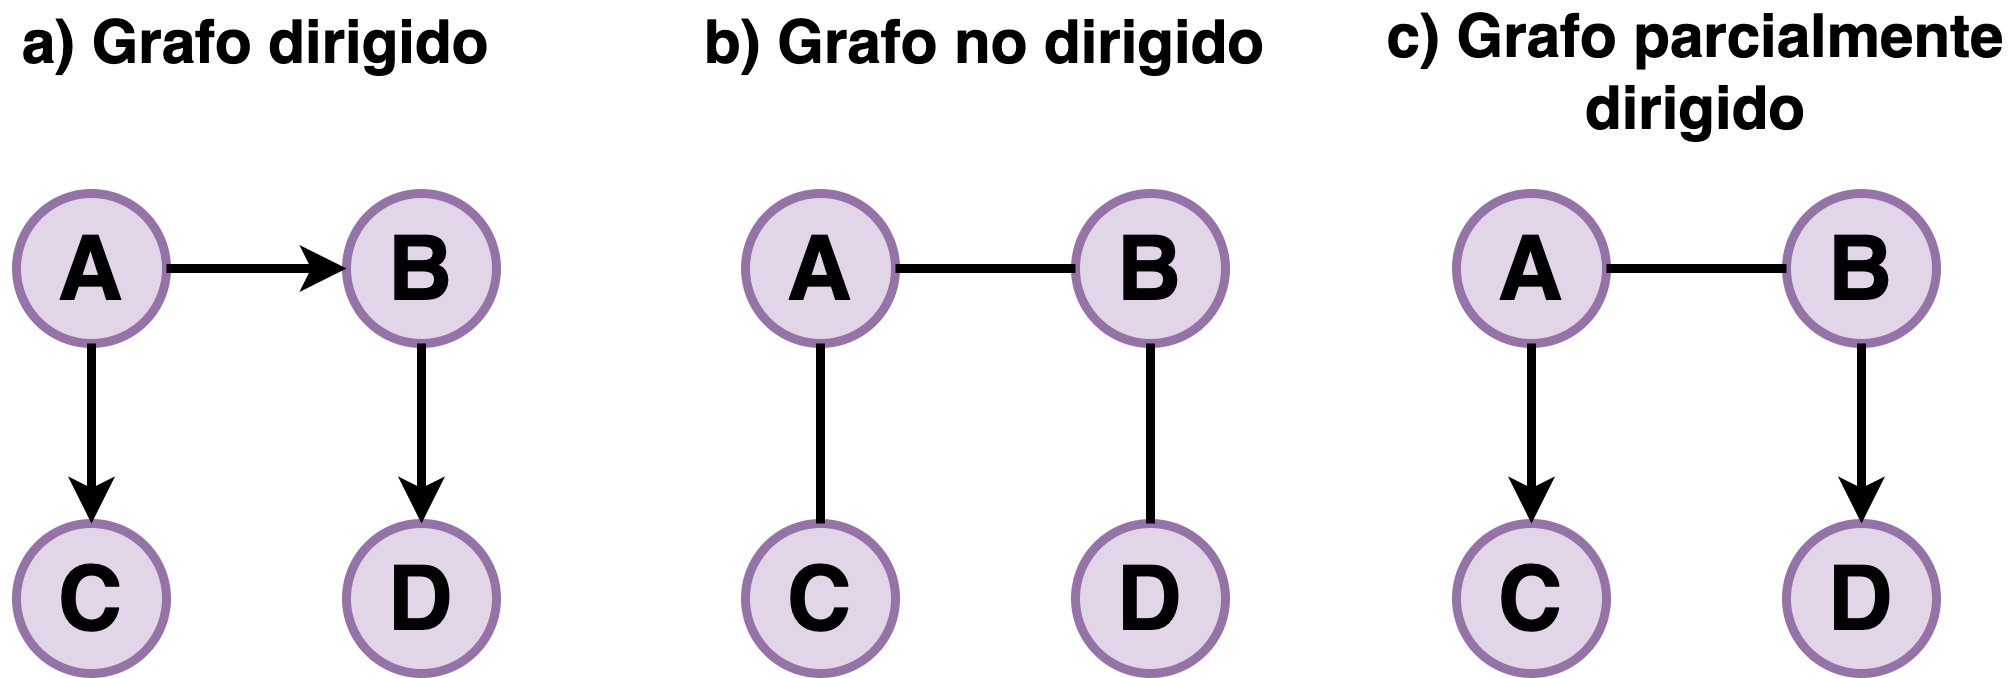
\includegraphics[scale=0.15]{figuras/fig1.png}
    % \caption[Así aparece el rótulo en el índice]{Así aparece el rótulo en el texto.}
    \caption[Tipos de grafos]{\textbf{Tipos de grafos.}}
    \label{fig1}
\end{figure}

La tabla~\ref{tab1} muestra...

\begin{table}[ht!]
\centering
\resizebox{\textwidth}{!}{
\begin{tabular}{@{}ccccc@{}}
\toprule
\textbf{Columna 1} & \textbf{Columna 2} & \textbf{Columna 3} & \textbf{Columna 4} & \textbf{Columna 5} \\ \midrule
Fila 1             & A                  & B                  & C                  & D                  \\ \midrule
Fila 2             & E                  & F                  & G                  & H                  \\ \midrule
Fila 3             & I                  & J                  & K                  & L                  \\ \bottomrule
\end{tabular}
}
% \caption[Así aparece el rótulo en el índice]{Así aparece el rótulo en el texto.}
\caption[Ejemplo de tabla]{\textbf{Ejemplo de tabla.}}
\label{tab1}
\end{table}


\subsection{Una subsubsección}
\label{una-subsubseccion}

El algoritmo~\ref{alg1} muestra...
\medskip

\begin{algorithm}[H]
\label{alg1}
\SetAlgoLined
\medskip
\begin{enumerate}
    \item Elegir una estructura de red $\mathcal{G}$ sobre $\mathbf{V}$, normalmente vacía. Establecer la puntuación máxima inicial: $Score_{max} = Score_{\mathcal{G}}$.
    \item Repetir los siguientes pasos mientras $Score_{max}$ siga aumentando:
    \begin{enumerate}
        \item Calcular las puntuaciones para todas las posibles redes modificadas $\mathcal{G}^{*}$ que se pueden obtener añadiendo, eliminando o reorientando un solo eje de $\mathcal{G}$ sin que se producan ciclos.
        \item Si para alguna de las redes modificadas $\mathcal{G}^{*}$ se cumple que $Score_{G^{*}} > Score_{\mathcal{G}}$, establecer $G = G^{*}$ y $Score_{max} = Score_{G^{*}}$.
    \end{enumerate}
    \item Devolver el DAG $\mathcal{G}$.
\end{enumerate}
 \caption{Algoritmo \textit{Hill-Climbing} (HC)}
\end{algorithm}


\newpage

Ejemplo de fórmula:

\begin{equation*}
    N_{k}(\mathbf{\mu},\mathbf{\Sigma}) = \frac{1}{\sqrt{2\pi\det(\Sigma})} \exp \bigg\{ -\frac{1}{2}(\mathbf{X}-\mathbf{\mu})^{T}\Sigma^{-1}(\mathbf{X}-\mathbf{\mu}) \bigg\} \quad \mathbf{X},\mathbf{\mu} \in \mathbb{R}^{k}
\end{equation*}

Otro ejemplo de fórmula:

\begin{equation*}
    \underbrace{P(\mathcal{B}|\mathcal{D}) = P(\mathcal{\mathcal{G}},\Theta|\mathcal{D})}_{\textbf{Aprendizaje}} = \underbrace{P(\mathcal{G}|\mathcal{D})}_{\textbf{Aprendizaje estructural}} \cdot \underbrace{P(\Theta|\mathcal{G},\mathcal{D})}_{\textbf{Aprendizaje paramétrico}}
\end{equation*}
